\indent\underline{\textbf{Ejercicio 4}}\\
En el Ejemplo 4.3 (\textit{Gambler’s problem, Sutton\&Barto, 2018})~\cite{Sutton2018}, la política óptima tiene una forma particular (ver figura~\ref{fig:gamblers_problem}) con máximo en $50$.
Es decir, cuando el jugador tiene $\$50$, le conviene apostarlo todo; sin embargo, cuando tiene $\$51$, le conviene apostar $\$1$.
¿Por qué sucede esto?

\begin{figure}[H]
    \centering
    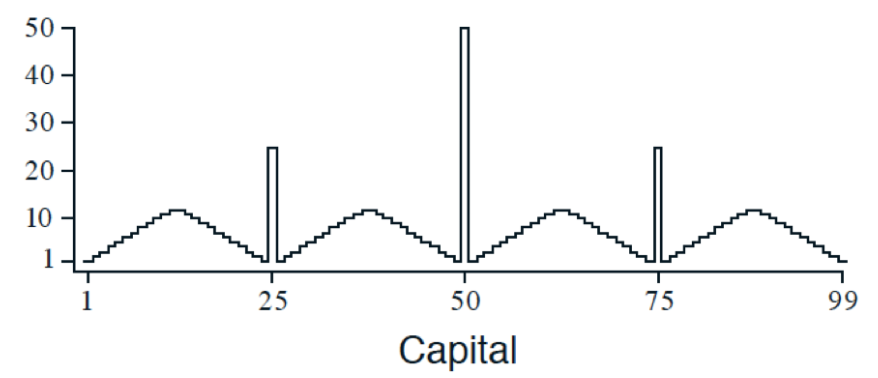
\includegraphics[width=0.5\textwidth]{../img/gamblers_problem}
    \caption{Ejemplo 4.3~\cite{Sutton2018}}
    \label{fig:gamblers_problem}
\end{figure}

\indent\underline{\textbf{Solución}}\\
El ejemplo 4.3 (\textit{Gambler’s problem, Sutton\&Barto, 2018})~\cite{Sutton2018} se plantea como un MDP finito, sin descuento, episódico y con un conjunto de estados $s \in \left\{0, 1, \ldots, 99\right\}$ y un conjunto de acciones $a \in \left\{0, 1, \ldots, \min(s, 100-s)\right\}$.

Por otro lado, la política final encontrada es tal que $p_h=0.4$, es decir, la probabilidad de que la moneda salga cara es $0.4$.

Por lo tanto, cuando la moneda está cargada y al jugador le conviene minimizar el número de apuestas realizadas porque en el largo plazo, el jugador perderá dinero.
Por lo tanto, el jugador tiene una \textit{ventaja}\footnotemark y le conviene apostar todo cuando tiene $\$50$, ya que a la izquierda y derecha de este valor las apuestas llevarán al jugador de vuelta a $\$50$.
Por lo que si tiene $\$51$ le conviene apostar $\$1$ sabiendo que si pierde, volverá a $\$50$.
\footnotetext{La ventaja se refiere a que si el jugador apuesta los $\$50$ tendrá el $40\%$ de probabilidad de ganar.}

\line(1,0){\textwidth}
